%%%%%%%%%%%%%%%%%%%%%%%%%%%%%%%%%%%%%%%%%
% Beamer Presentation
% LaTeX Template
% Version 1.0 (10/11/12)
%
% This template has been downloaded from:
% http://www.LaTeXTemplates.com
%
% License:
% CC BY-NC-SA 3.0 (http://creativecommons.org/licenses/by-nc-sa/3.0/)
%
%%%%%%%%%%%%%%%%%%%%%%%%%%%%%%%%%%%%%%%%%

%----------------------------------------------------------------------------------------
%	PACKAGES AND THEMES
%----------------------------------------------------------------------------------------

\documentclass{beamer}

\mode<presentation> {

% The Beamer class comes with a number of default slide themes
% which change the colors and layouts of slides. Below this is a list
% of all the themes, uncomment each in turn to see what they look like.

% \usetheme{default}
% \usetheme{AnnArbor}
% \usetheme{Antibes}
% \usetheme{Bergen}
% \usetheme{Berkeley}
% \usetheme{Berlin}
% \usetheme{Boadilla}
% \usetheme{CambridgeUS}
% \usetheme{Copenhagen}
% \usetheme{Darmstadt}
% \usetheme{Dresden}
% \usetheme{Frankfurt}
% \usetheme{Goettingen}
% \usetheme{Hannover}
% \usetheme{Ilmenau}
% \usetheme{JuanLesPins}
% \usetheme{Luebeck} % nice
\usetheme{Madrid}   % nice
% \usetheme{Malmoe} % nicer
% \usetheme{Marburg}
% \usetheme{Montpellier}
% \usetheme{PaloAlto}
% \usetheme{Pittsburgh}
% \usetheme{Rochester} % Plain
% \usetheme{Singapore}
% \usetheme{Szeged}
% \usetheme{Warsaw}

% As well as themes, the Beamer class has a number of color themes
% for any slide theme. Uncomment each of these in turn to see how it
% changes the colors of your current slide theme.

% \usecolortheme{albatross}
% \usecolortheme{beaver}
% \usecolortheme{beetle}
% \usecolortheme{crane}
% \usecolortheme{dolphin}
% \usecolortheme{dove}
% \usecolortheme{fly}
% \usecolortheme{lily}
% \usecolortheme{orchid}
% \usecolortheme{rose}
% \usecolortheme{seagull}
% \usecolortheme{seahorse}
% \usecolortheme{whale}
% \usecolortheme{wolverine}

%\setbeamertemplate{footline} % To remove the footer line in all slides uncomment this line
%\setbeamertemplate{footline}[page number] % To replace the footer line in all slides with a simple slide count uncomment this line

\setbeamertemplate{navigation symbols}{} % To remove the navigation symbols from the bottom of all slides uncomment this line
}

\AtBeginSection[]{%
  \begin{frame}
    \frametitle{Plan}
    \tableofcontents[currentsection]
  \end{frame}
}


\usepackage{graphicx} % Allows including images
\usepackage{booktabs} % Allows the use of \toprule, \midrule and \bottomrule in tables
\usepackage{calc, relsize}

\usepackage{proof, mathpartir}

\usepackage{tikz}
\usetikzlibrary{
  shapes,
  positioning,
  arrows,
  arrows.meta,
  overlay-beamer-styles, % from aobs-tikz for beamer overlays in tikzpictures
}


\tikzstyle{process}=[circle,thick,draw=blue!75,minimum size=6mm]
\tikzstyle{channel}=[>={Stealth[width=7pt, length=6pt]}]
\tikzstyle{label}=[midway, above, font=\relsize{-1.5}]
\tikzstyle{message}=[>={Stealth[width=7pt, length=6pt]}]
\tikzstyle{message-label}=[midway, above, font=\relsize{-2}, text=green]


%----------------------------------------------------------------------------------------
%	SPECIFIC PACKAGES
%----------------------------------------------------------------------------------------

\newcommand\indexVar{k}
\newcommand\lab{lab}

\usepackage{macro/generic}
\usepackage[index=\indexVar,label=\lab]{../macro/language}
\usepackage{macro/code}


%----------------------------------------------------------------------------------------
%	MACROS
%----------------------------------------------------------------------------------------

\newcommand\shift[1]{1.5em / {1.0 / \real{#1}}} % Does not work, try to fix
\newcommand\polyvar[1]{\color{red}{#1}}


%----------------------------------------------------------------------------------------
%	TITLE PAGE
%----------------------------------------------------------------------------------------

\title[Intersections and Unions of Session Types]{Intersections and Unions of Session Types} % The short title appears at the bottom of every slide, the full title is only on the title page

\author[C. Acay \& F. Pfenning]{
  Co\c{s}ku Acay
  \and
  Frank Pfenning
}
\institute[CMU] % Your institution as it will appear on the bottom of every slide, may be shorthand to save space
{
Carnegie Mellon University \\ % Your institution for the title page
School of Computer Science
}
\date{ITRS 2016} % Date, can be changed to a custom date

\begin{document}

\begin{frame}
\titlepage % Print the title page as the first slide
\end{frame}

\begin{frame}
\frametitle{Overview} % Table of contents slide, comment this block out to remove it
\tableofcontents % Throughout your presentation, if you choose to use \section{} and \subsection{} commands, these will automatically be printed on this slide as an overview of your presentation
\end{frame}

%----------------------------------------------------------------------------------------
%	PRESENTATION SLIDES
%----------------------------------------------------------------------------------------

%------------------------------------------------
\section{Background}
%------------------------------------------------

\subsection{Message-passing Concurrency}

\begin{frame}[fragile]
  \frametitle{Setting}
  \begin{itemize}
    \item Processes represented as nodes
    \item Channels go between processes and represented as edges
    \item Each channel is ``provided'' by a specific process (e.g.\ $P$ provides $c$, $Q$ provides $d$ etc.): one-to-one correspondence between channels and processes
  \end{itemize}

  \medskip

  \begin{center}
  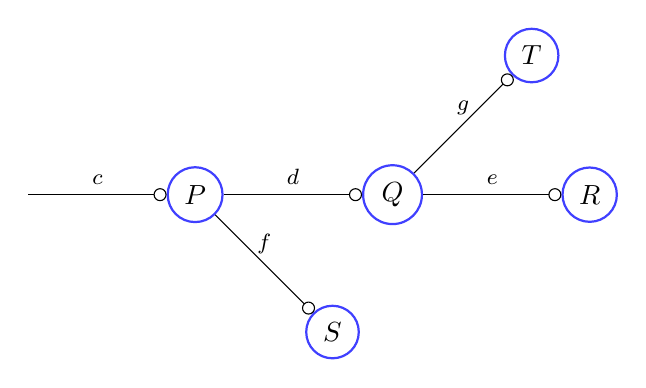
\begin{tikzpicture}[node distance=5em]
    \node[process] (P) {$P$};
    \node[process, right=of P] (Q) {$Q$};
    \node[process, right=of Q] (R) {$R$};
    \node[process, below right=of P] (S) {$S$};
    \node[process, above right=of Q] (T) {$T$};
    \coordinate[left=of P] (p);

    \draw[channel, -o] (p) to node [label] (c) {$c$} (P);
    \draw[channel, -o] (P) to node [label] (d) {$d$} (Q);
    \draw[channel, -o] (Q) to node [label] (e) {$e$} (R);
    \draw[channel, -o] (P) to node [label] (f) {$f$} (S);
    \draw[channel, -o] (Q) to node [label] (g) {$g$} (T);
  \end{tikzpicture}
  \end{center}

\end{frame}

%------------------------------------------------

\begin{frame}[fragile]
  \frametitle{Communication}
  \begin{itemize}
    \item Processes compute internally
    \item Exchange messages along channels
  \end{itemize}

  \bigskip

  \begin{center}
  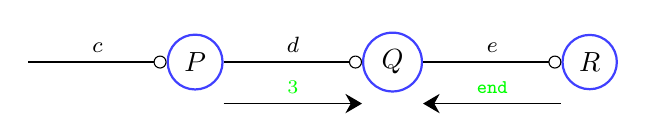
\begin{tikzpicture}[node distance=5em]
    \node[process] (P) {$P$};
    \node[process, right=of P] (Q) {$Q$};
    \node[process, right=of Q, visible on=<-3>] (R) {$R$};
    \coordinate[left=of P] (p);

    \draw[channel, -o] (p) to node [label] (c) {$c$} (P);
    \draw[channel, -o] (P) to node [label] (d) {$d$} (Q);
    \draw[channel, -o, visible on=<-3>] (Q) to node [label] (e) {$e$} (R);

    \pause
    \draw[message, ->, transform canvas={yshift=-1.5em}] (P) to
      node [message-label] {3} (Q);

    \pause
    \draw[message, <-, transform canvas={yshift=-3em}] (P) to
      node [message-label] {\qquote{aaa}} (Q);

    \draw[message, <-, transform canvas={yshift=-1.5em}, visible on=<3>] (Q) to
      node [message-label] {\texttt{end}} (R);

    \pause
  \end{tikzpicture}
  \end{center}

  \bigskip\bigskip
  \only<4>{\par \footnotesize{$^*$Note that communication is synchronous.}}

\end{frame}

%------------------------------------------------

\begin{frame}[fragile]
  \frametitle{Higher-order Messages}
  \begin{itemize}
    \item Processes can also send channels they own
  \end{itemize}

  \bigskip

  \begin{center}
  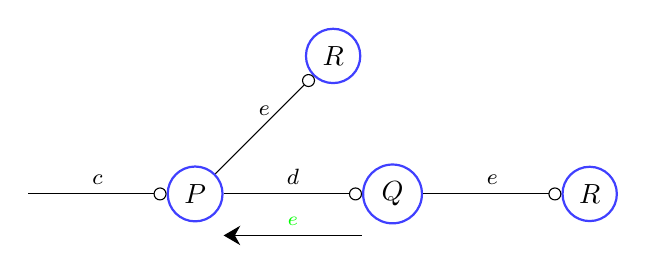
\begin{tikzpicture}[node distance=5em]
    \node[process] (P) {$P$};
    \node[process, right=of P] (Q) {$Q$};
    \node[process, right=of Q, visible on=<-2>] (R) {$R$};
    \node[process, above right=of P, visible on=<3>] (R2) {$R$};
    \coordinate[left=of P] (p);

    \draw[channel, -o] (p) to node [label] (c) {$c$} (P);
    \draw[channel, -o] (P) to node [label] (d) {$d$} (Q);
    \draw[channel, -o, visible on=<-2>] (Q) to node [label] (e) {$e$} (R);
    \draw[channel, -o, visible on=<3>] (P) to node [label] (e2) {$e$} (R2);

    \pause
    \draw[message, <-, transform canvas={yshift=-1.5em}] (P) to
      node [message-label] {$e$} (Q);

    \pause

  \end{tikzpicture}
  \end{center}

\end{frame}

%------------------------------------------------

\subsection{Session Types}

%------------------------------------------------

\begin{frame}[fragile]
  \frametitle{Session Types}
  \begin{itemize}
    \item Don't want to send \texttt{int} if expecting \texttt{string}
    \item Don't try to receive if other process is not sending
  \end{itemize}

  \medskip
  \pause
  \par \textbf{Solution: Assign types to each channel}
  \pause
  (from provider's perspective).

  \bigskip

  \pause

  \begin{center}
  \begin{tikzpicture}[node distance=7em]
    \node[process] (P) {$P$};
    \node[process, right=of P] (Q) {$Q$};
    \node[process, right=of Q, visible on=<4-7>] (R) {$R$};
    \coordinate[left=of P] (p);

    \draw[channel, -o] (p) to node [label] (c) {$c : \polyvar{A}$} (P);
    \draw[channel, -o, visible on=<4>] (P) to node [label] (d) {$d : \texttt{int} \recvVal \texttt{string} \sendVal \polyvar{B}$} (Q);
    \draw[channel, -o, visible on=<5>] (P) to node [label] (d) {$d : \texttt{string} \sendVal \polyvar{B}$} (Q);
    \draw[channel, -o, visible on=<6->] (P) to node [label] (d) {$d : \polyvar{B}$} (Q);
    \draw[channel, -o, visible on=<4-7>] (Q) to node [label] (e) {$e : \terminate$} (R);

    \pause
    \draw[message, ->, transform canvas={yshift=-1.5em}] (P) to
      node [message-label] {3} (Q);

    \pause
    \draw[message, <-, transform canvas={yshift=-3em}] (P) to
      node [message-label] {\qquote{aaa}} (Q);

    \pause

    \draw[message, <-, transform canvas={yshift=-1.5em}, visible on=<7>] (Q) to
      node [message-label] {\texttt{end}} (R);

    \pause
  \end{tikzpicture}
  \end{center}

\end{frame}

%------------------------------------------------

\begin{frame}
  \frametitle{Why linear?}
  \begin{itemize}
    \item Sessions are resources: communicating along a channel consumes the old type
    \item Contraction would violate type safety
    \item Weakening would work, but we keep things simple
  \end{itemize}
\end{frame}

%------------------------------------------------

\begin{frame}[fragile]
  \frametitle{Linear Propositions as Session Types}
  \begin{center}
  \begin{tabular}{l l}
      $\terminate$        & send \texttt{end} and terminate \\
      $A \tensor B$       & send channel of type $A$ and continue as $B$ \\
      $\tau \sendVal B$   & send value of type $\tau$ and continue as $B$ \\
      $\internals{A}{I}$  & send $\lab_i$ and continue as $A_i$ for some $i \in I$\\
      $A \lolli B$        & receive channel of type $A$ and continue as $B$ \\
      $\tau \recvVal B$   & receive value of type $\tau$ and continue as $B$ \\
      $\externals{A}{I}$  & receive $\lab_i$ and continue as $A_i$ for some $i \in I$ \\
      $\recursive t {A_t}$ & (equi-)recursive type
  \end{tabular}
  \end{center}

  \pause

  \bigskip
  \textbf{Example: Queue Interface}

  \begin{lstlisting}
type queue = &{ enq : A -o queue
              , deg : +{none : 1, some : A * queue}
              }
  \end{lstlisting}
\end{frame}

%------------------------------------------------

\begin{frame}
  \frametitle{Proof Terms as Concurrent Processes}

  $P, Q, R$ ::=
  \begin{center}
  \begin{tabular}{l l}
    $\tspawn{x}{P_x}{Q_x}$     & cut (spawn) \\
    $\tfwd c d$                & id (forward) \\
    $\tclose c \mid \twait c P$  & $\terminate$ \\
    $\tsend{c}{y}{P_y}{Q} \mid \trecv{x}{c}{R_x}$ & $A \tensor B,$ $A \lolli B$ \\
    $\tselect{c}{}{P} \mid \tcase c {\tbranches Q I}$  & $\externals A I,$ $\internals A I$
  \end{tabular}
  \end{center}
\end{frame}

%------------------------------------------------

\begin{frame}[fragile]
  \frametitle{Example: An Implementation of Queues}
  \begin{lstlisting}
type queue = &{ enq : A -o queue
              , deg : +{none : 1, some : A * queue}
              }
  \end{lstlisting}

  \begin{center}
  \begin{tabular}{c}
  \begin{lstlisting}
empty : queue
q <- empty = case q of
  enq -> x <- recv q;
         e <- empty;
         q <- elem x e
  deq -> q.none; close q

elem : A -o queue -o queue
q <- elem x r = case q of
  enq -> y <- recv q;
         r.enq; send r y;
         q <- elem x r
  deq -> q.some; send q x;
         q <- r
  \end{lstlisting}
  \end{tabular}
  \end{center}
\end{frame}

%------------------------------------------------

\begin{frame}[fragile]
  \frametitle{Process Typing}
  Typing judgement has the form $\typeRecDJ P c A$ meaning ``process $P$ offers along channel $c$ the session $A$ under the context $\ctx$.'' $\recCtx$ tracks recursive variables.

  \pause
  \bigskip
  Some examples:

\begin{mathpar}
  % id and cut
  \infer[\id]{ \typeD {c : A} {\tfwd{d}{c}} {d} {A} }
    {}
  \and \infer[\cut]{ \typeD {\ctx, \ctx'} {\tspawn{c}{P_c}{Q_c}} {d} {D} }
    { \typeD {\ctx} {P_c} {c} {A}
    & \typeD {\ctx', c : A} {Q_c} {d} {D}
    }
  % Terminate
  \and \infer[\terminate\Right]{\typeD{\emptyCtx}{\tclose c}{c}{\terminate}}
    {}
  \and \infer[\terminate\Left]{\typeD{\ctx, c : \terminate}{\twait c P}{d}{A}}
    {\typeDJ{P}{d}{A}}
  % Tensor
  \and \infer[\tensor\Right]{\typeD{\ctx, \ctx'}{\tsend{c}{d}{P_d}{Q}}{c}{A \tensor B}}
    { \typeD{\ctx}{P}{d}{A}
    & \typeD{\ctx'}{Q}{c}{B}
    }
\end{mathpar}
\end{frame}


%------------------------------------------------
\subsection{Subtyping}
%------------------------------------------------


\begin{frame}[fragile]
  \frametitle{Subtyping}
  \begin{itemize}
    \item Width and depth subtyping for $n$-ary choices
    \item Width: $\externals A I \sub \externals A J$ whenever $J \subseteq I$
    \item Depth: $\externals A I \sub \externals {A'} I$ whenever $A_i \sub A'_i$
    \pause
    \item Defined coinductively because of recursive types
  \end{itemize}

  \pause

  \bigskip
  Introduced to process typing using subsumption:
  \begin{mathpar}
    \infer[\irb{Sub}\Right]{\typeRecDJ{P}{c}{A}}
      {\typeRecDJ{P}{c}{A'} & A' \sub A}
    \and \infer[\irb{Sub}\Left]{\typeRecD {\ctx, c : A} \recCtx P d B}
      {\typeRecD{\ctx, c : A'} {\recCtx} P d B & A \sub A'}
  \end{mathpar}
\end{frame}

%------------------------------------------------
\subsection{Configurations and Reduction}
%------------------------------------------------

\begin{frame}
  \frametitle{Configurations}
  \begin{itemize}
    \item A processes by itself is not very useful in concurrent setting
    \item Need to be able to talk about interactions
    \pause
    \item Use a process configuration, which is simply a set of labelled processes: $\config = {\proc {c_1} {P_1}, \ldots, \proc {c_n} {P_n}}$.
    \pause
    \item Typing judgement, $\providesCtx \config \ctx$, imposes a tree structure (ensures linearity)
  \end{itemize}
\end{frame}

%------------------------------------------------

\begin{frame}[fragile]
  \frametitle{Reduction}
  Configurations reduce by interaction. Some examples:

  \bigskip

  \begin{align*}
    % Id
    \irb{id}     \hspace{1em} & : \proc{c}{\tfwd{c}{d}} \lolli \monad{c = d} \\
    % Cut
    \irb{cut}    \hspace{1em} & : \proc{c}{\tspawn{x}{P_x}{Q_x}}
        \lolli \monad{\exists a. \proc{a}{P_a} \otimes \proc{c}{Q_a}} \\
    % One
    \irb{one} \hspace{1em} & : \proc{c}{\tclose{c}} \otimes \proc{d}{\twait{c}{P}}
      \lolli \monad{\proc{d}{P}}
  \end{align*}

\end{frame}


%------------------------------------------------
\section{Intersections and Unions}
%------------------------------------------------


\begin{frame}[fragile]
  \frametitle{Intersections and Unions}

  \par What if we want to track more properties of queues?
  \pause
  Empty, non-empty, even length?

  \pause
  \bigskip
  \par These can be defined in the base system:

  \bigskip

  \begin{lstlisting}
type empty-queue = &{ enq : A -o queue
                    , deg : +{none : 1}
                    }

type nonempty-queue = &{ enq : A -o queue
                       , deg : +{some : A * queue}
                       }
  \end{lstlisting}

\pause
\bigskip
\textbf{However, there is no way to properly track them!}

\end{frame}

%------------------------------------------------

\begin{frame}[fragile]
  \textbf{We cannot track multiple refinements.}
  \pause
  Consider \lstinline$concat : queue -o queue -o queue$ that concatenates two queues. It has many types but no most general type:

  \bigskip

  \begin{lstlisting}
concat : empty-queue -o empty-queue -o empty-queue
concat : queue -o nonempty-queue -o nonempty-queue
concat : nonempty-queue -o queue -o nonempty-queue
  \end{lstlisting}
\end{frame}

%------------------------------------------------
\subsection{Intersection Types}
%------------------------------------------------

\begin{frame}
  \frametitle{Intersection Types}
  \begin{itemize}
    \item Intersection of two types: $A \intersect B$
    \item $c : A \intersect B$ if channel c offers both behaviors simultaneously
  \end{itemize}

  \pause
  \bigskip

  \begin{mathpar}
    \infer[\intersect\Right]{\typeRecDJ{P}{c}{A \intersect B}}
      {\typeRecDJ{P}{c}{A} & \typeRecDJ{P}{c}{B}}
    \and\infer[\intersect\Left_1]{\typeRecD{\ctx, c : A \intersect B}{\recCtx}{P}{d}{D}}
      {\typeRecD{\ctx, c : A}{\recCtx}{P}{d}{D}}
    \and \infer[\intersect\Left_2]{\typeRecD{\ctx, c : A \intersect B}{\recCtx}{P}{d}{D}}
      {\typeRecD{\ctx, c : B}{\recCtx}{P}{d}{D}}
  \end{mathpar}
\end{frame}

%------------------------------------------------

\begin{frame}[fragile]
  \frametitle{Intersections Solve the Previous Problem}
   We can now specify multiple behavioral properties:

   \bigskip

  \begin{lstlisting}
concat : empty-queue -o empty-queue -o empty-queue
     and queue -o nonempty-queue -o nonempty-queue
     and nonempty-queue -o queue -o nonempty-queue
  \end{lstlisting}

\end{frame}

%------------------------------------------------
\subsection{Union Types}
%------------------------------------------------

\begin{frame}
  \frametitle{Union Types}
  \begin{itemize}
    \item Union of two types: $A \union B$
    \item $c : A \union B$ if channel c offers either behavior
    \pause
    \item Dual to intersections
  \end{itemize}

  \pause
  \bigskip

  \begin{mathpar}
    \infer[\union\Right_1]{\typeRecDJ{P}{c}{A \union B}}
      {\typeRecDJ{P}{c}{A}}
    \and \infer[\union\Right_2]{\typeRecDJ{P}{c}{A \union B}}
      {\typeRecDJ{P}{c}{B}}
    \and \infer[\union\Left]{\typeRecD{\ctx, c : A \union B}{\recCtx}{P}{d}{D}}
      {\typeRecD{\ctx, c : A}{\recCtx}{P}{d}{D} & \typeRecD{\ctx, c : B}{\recCtx}{P}{d}{D}}
  \end{mathpar}
\end{frame}

%------------------------------------------------

\begin{frame}[fragile]
  \frametitle{Reasons for Adding Unions}
  \begin{itemize}
    \item Maintain the symmetry of the system
    \item Makes working with internal choice more convenient
    \item Interpretation of internal choice (we will explain later)
  \end{itemize}

  \pause
  \bigskip
  We can also write things like:
  \bigskip

  \begin{lstlisting}
type queue = empty-queue or nonempty-queue
  \end{lstlisting}

\end{frame}

%------------------------------------------------
\subsection{Reinterpreting Choice}
%------------------------------------------------

\begin{frame}
  \frametitle{Reinterpreting Choice}
  Consider $\external\braces{\irb{inl} : A, \irb{inr} : B}$

  \pause
  \bigskip
  This type says: ``I will act as $A$ if you send me $\irb{inl}$ \emph{and} I will act as $B$ if you send me $\irb{inr}$.''

  \pause
  \bigskip
  Interpreting \emph{and} as $\intersect$ gives $\external\braces{\irb{inl} : A, \irb{inr} : B} \approx \externalSing {\irb{inl}} A \intersect \externalSing {\irb{inr}} B$.
\end{frame}

%------------------------------------------------

\begin{frame}[fragile]
  \frametitle{Reinterpreting Choice - General Case}
  Generalizing to $n$-ary choice and dualising gives:

  \medskip

  \begin{mathpar}
    \externals A I \defined \bigintersect_{\indexVar \in I}{\external\braces{\lab_\indexVar : A_\indexVar}} \\
    \internals A I \defined \bigunion_{\indexVar \in I}{\internal\braces{\lab_\indexVar : A_\indexVar}}
  \end{mathpar}

  \bigskip
  Easy to verify these definitions satisfy the typing rules.

  \pause
  \bigskip
  Suggests treating intersections and unions as implicit choice.
\end{frame}

%------------------------------------------------
\section{Algorithmic System}
%------------------------------------------------

\begin{frame}[fragile]
  \frametitle{Algorithmic Subtyping}
  Idea: make $\Sub{\intersect\Left_{\set{1,2}}}$ and $\Sub{\union\Right_{\set{1,2}}}$ invertible so we can apply eagerly.

  \medskip

  \bgroup
  \def\arraystretch{3}
  \begin{center}
  \begin{tabular}{l c l}
    $ \infer=[\Sub{\intersect\Left_{\set{1,2}}}]{A_1 \intersect A_2 \sub B}
       {A_{\set{1,2}} \sub B}
    $
    & $\longrightarrow$
    & $ \infer=[\SubA{\intersect}\Left]{\typeList, A_1 \intersect A_2 \subA \typeListB}
         {\typeList, A_1, A_2 \subA \typeListB}
      $
    \\
    $ \infer=[\Sub{\union\Right_{\set{1,2}}}]{A \sub B_1 \union B_2}
       {A \sub B_{\set{1,2}}}
    $
    & $\longrightarrow$
    & $ \infer=[\SubA{\union}\Right]{\typeList \subA \typeListB, A_1 \union A_2}
         {\typeList \subA \typeListB, A_1, A_2}
      $
  \end{tabular}
  \end{center}
  \egroup

  \pause
  \medskip
  Also admits distributivity:
  \begin{mathpar}
     (A_1 \union B) \intersect (A_2 \union B) \typeeq (A_1 \intersect A_2) \union B \\
     (A_1 \union A_2) \intersect B \typeeq (A_1 \intersect B) \union (A_2 \intersect B)
  \end{mathpar}
  Turns out to be necessary for soundness of algorithmic typing.
\end{frame}

%------------------------------------------------

\begin{frame}[fragile]
  \frametitle{Algorithmic Type Checking}
  \begin{itemize}
    \item Make $\intersect\Left_{\set{1,2}}$ and $\union\Right_{\set{1,2}}$ invertible so we can apply eagerly.
    \pause
    \item Delay subtyping to $\irb{id}$
    \item Label $\irb{cut}$ with it's type
  \end{itemize}

  \pause
  \smallskip

  \bgroup
  \def\arraystretch{3}
  \begin{center}
  \begin{tabular}{l c l}
    \footnotesize
    $ \infer[\intersect\Left_{1,2}]{\typeRecD{\ctx, c : A_1 \intersect A_2}{\recCtx}{P}{d}{D}}
       {\typeRecD{\ctx, c : A_{1,2}}{\recCtx}{P}{d}{D}}
    $
    & $\rightarrow$
    & $ \infer[\intersect\Left]{\typeRecAJR{\ctx, c : (\typeList, A \intersect B)}{P}{d}{\typeListB}}
         {\typeRecAJR{\ctx, c : (\typeList, A, B)}{P}{d}{\typeListB}}
      $
    \\
    $ \infer[\union\Right_{1,2}]{\typeRecDJ{P}{c}{A_1 \union A_2}}
       {\typeRecDJ{P}{c}{A_{1,2}}}
    $
    & $\rightarrow$
    & $ \infer[\union\Right]{\typeRecAJR \ctx P c {A \union B, \typeList}}
         {\typeRecAJR \ctx P c {A, B, \typeList}}
      $
  \end{tabular}
  \end{center}
  \egroup

  \pause

  \begin{mathpar}
  % id and cut
    \infer[\id]{ \typeRecAJR {c : \typeList} {\tfwd d c} {d} {\typeListB} }
      { \typeList \subA \typeListB }
    \and \infer[\cut]{ \typeRecAJR {\ctx, \ctx'} {\tspawnType c {P_c} A {Q_c}} {d} \typeList }
      { \typeRecAJR \ctx {P_c} {c} {A}
      & \typeRecAJR {\ctx', c : A} {Q_c} {d} {\typeList}
      }
  \end{mathpar}
\end{frame}

%------------------------------------------------

\begin{frame}
  \frametitle{Results}
  \begin{theorem}[Completeness of Algorithmic Subtyping]
  Algorithmic subtyping is complete with respect to declarative subtyping.
  \end{theorem}

  \bigskip

  \begin{theorem}[Equivalence of Algorithmic Typing]
  Algorithmic typing is sound and complete with respect to declarative typing.
  \end{theorem}
\end{frame}

%------------------------------------------------
\section{Metatheory}
%------------------------------------------------

\begin{frame}
  \frametitle{Type Safety}
  We have proved progress and preservation for the system extended with intersections and unions.

  \pause
  \bigskip
  Progress $\rightarrow$ deadlock-freedom

  \bigskip
  Type preservation $\rightarrow$ session fidelity
\end{frame}

%------------------------------------------------

\begin{frame}
  \frametitle{Progress}
  \begin{theorem}[Progress]
    If $\providesCtx \config \ctx$ then either
    \begin{enumerate}
      \item $\steps{\config}{\config'}$ for some $\config'$, or
      \item $\config$ is poised$^*$.
    \end{enumerate}
  \end{theorem}
  \begin{proof}
    By induction on $\providesCtx \config \ctx$ followed by a nested induction on the typing of the root process. When two processes are involved, we also need inversion on client's typing.
  \end{proof}

\bigskip

$^*$A process is poised if it is waiting to communicate with its client.

\end{frame}

%------------------------------------------------

\begin{frame}
  \frametitle{Type Preservation}
  \begin{theorem}[Preservation]
    If $\providesCtx \config \ctx$ and $\steps{\config}{\config'}$ then $\providesCtx {\config'} \ctx$.
  \end{theorem}
\begin{proof}
  By inversion on $\steps{\config}{\config'}$, followed by induction on the typing judgments of the involved processes. Each branch requires a hand-rolled induction hypothesis.
\end{proof}

\end{frame}

%------------------------------------------------

\begin{frame}
  \frametitle{Conclusion and Highlights}
  We introduced intersection and union types to a session-typed process calculus and demonstrated their usefulness.

  \bigskip
  \begin{itemize}
    \item Unions work naturally. The elimination rule we give has been shown unsound in the presence of effects (even non-termination).
    \pause
    \item More general than refinement system of Freeman and Pfenning
    \pause
    \item Subtyping resembles Gentzen's multiple conclusion calculus
    \pause
    \item Algorithmic typing mirrors subtyping
  \end{itemize}
\end{frame}

%------------------------------------------------

\begin{frame}
  \frametitle{Future Work}
  \begin{itemize}
    \item Simple: integrate a functional language, extend to shared channels and asynchronous communication
    \pause
    \item More interesting: Add polymorphism and abstract types
    \begin{itemize}
      \item Polymorphism is non-trivial with equirecursive types
    \end{itemize}
    \pause
    \item Applications other than refinements?
  \end{itemize}
\end{frame}

%------------------------------------------------

\begin{frame}
\Huge{\centerline{The End}}
\end{frame}

%----------------------------------------------------------------------------------------

\end{document} 
